\documentclass[russian,ukrainian,utf8,floatsection,equationsingle,14pt,simple]{eskdtext}

% \usepackage{eskdchngsheet}
\usepackage[T2A]{fontenc}
\usepackage[utf8]{inputenc}
% \geometry{left=3cm}
%\usepackage{cyrtimes}
\usepackage{pscyr}
\usepackage{mathtext}
\usepackage{tabularx}
\usepackage{multirow}
\usepackage{listings}
\usepackage{setspace}
\usepackage{amsmath}
\usepackage{amssymb}
\usepackage{graphicx}
\usepackage{verbatim}
\usepackage{indentfirst}
\usepackage{lscape}
\usepackage{paralist}
\usepackage{gost}
\usepackage{longtable}
\usepackage[thmmarks,amsmath]{ntheorem}
\usepackage[unicode]{hyperref}
\usepackage[linesnumbered]{algorithm2e}

\usepackage{rotating}
\usepackage{ulem}
\usepackage{cancel}
%Чтобы ссылки автоматически не вставлялись под \path
\def\BibUrl#1{#1} 
% \ESKDsectStyle{section}{\Large\bfseries}
% \ESKDsectAlign{section}{Center}
\ESKDsectSkip{section}{5pt}{10pt}
\ESKDsectSkip{subsection}{5pt}{5pt}
\ESKDsectSkip{subsubsection}{0pt}{5pt}
\renewcommand{\baselinestretch}{1.5} % Задаём единичный межстрочный интервал

% vim: nocindent:

\hyphenation
{
  три-ва-лість
  Від-по-відь
  Open-FOAM
  ал-го-рит-мів
  ал-го-рит-мом
  ал-го-рит-му
  апро-кси-ма-ція-ми
  біб-ліо-те-ка
  век-тор
  век-то-ри
  век-то-рів
  виг-ля-ді
  від-нос-но
  від-по-ві-да-ють
  влас-ний
  влас-них
  вуз-ла
  вхід-них
  дея-кі
  до-дат-ко-ві
  ефек-тив-ним
  зас-то-со-вує-ться
  зруч-но-му
  ка-фед-рою
  квад-рат
  квад-рат-ної
  ква-лі-фі-ка-цій-но
  клас-тер-ної
  кое-фі-ці-єнт
  мак-си-маль-ної
  мат-ри-ці
  мат-риць
  мат-ри-ця
  мож-ли-вим
  нас-туп-ні
  не-мож-ли-во
  об-роб-ля-ти
  об-чис-ленні
  об-чис-лення
  об-чис-лень
  об-чис-лю-валь-ни-ми
  об-чис-лю-валь-но
  об-чис-лю-валь-ної
  пе-ре-тво-рен-ня
  пос-лі-дов-нос-ті
  прак-тич-не
  пре-фікс-ної
  про-дук-тив-ність
  різ-но-ма-ніт-них
  роз-рід-же-ної
  си-ме-трич-них
  си-ме-трич-ної
  сис-тем
  сис-те-мі
  склад-ність
  склад-но-сті
  цик-лу
}

\ESKDdepartment{Міністерство освіти і науки України}
\ESKDcompany{Національний технічний університет України%
<<Київський політехнічний інститут>>}

\ESKDauthor{Радер~Р.\,І.}
%\ESKDchecker{Стіренко~С.\,Г.}
%\ESKDnormContr{Симоненко~В.\,П.}
%\ESKDapprovedBy{Луцький~Г.\,М.}
\ESKDdate{2012/01/16}
\ESKDcolumnIX{НТУУ <<КПІ>> ФІОТ ІО-02}

% Set text padding
\ESKDsetPadding{10mm}{10mm}

% Redefine TOC styles
\makeatletter
\renewcommand{\l@section}{\@dottedtocline{0}{1.5em}{2.3em}}
\renewcommand{\l@subsection}{\@dottedtocline{1}{2.5em}{2.3em}}
\renewcommand{\l@subsubsection}{\@dottedtocline{2}{3.5em}{2.3em}}
\makeatother

% Document separator
\newcommand{\docseparator}[1]{
  \newpage
  \thispagestyle{empty}
  \ESKDthisStyle{empty}
  \noindent\parbox[c][\vsize][c]{\hsize}
  {\centering\fontsize{36pt}{40pt}\selectfont#1}

  % reset all counters
  \setcounter{page}{0}
  \setcounter{section}{0}
  \setcounter{subsection}{0}
  \setcounter{subsubsection}{0}
}

\newcommand{\apptitletop}[1]{%
ДОДАТОК #1\par
Алгоритм динамічної маршрутизації мультікастової розсилки}

\newcommand{\apptitlepages}[1]{%
Аркушів \pageref{LastPage}\par}

% Appendix title page
\newcommand{\appendixtitle}[3]{
  \newpage
  \thispagestyle{empty}
  \ESKDthisStyle{empty}
  \noindent
  \parbox[t][0.15\vsize][t]{\hsize}
  {\centering\large\apptitletop{#1}}
  \parbox[t][0.4\vsize][c]{\hsize}
  {\centering\Large\textbf{#2}\par#3}
  \parbox[t][0.20\vsize][c]{\hsize}{~~}
  \parbox[t][0.08\vsize][t]{\hsize}
  {\centering\apptitlepages}
  \vfill
  \noindent\parbox[c]{\hsize}{\centering\titlebottom}

  % reset all counters
  \setcounter{page}{0}
  \setcounter{section}{0}
  \setcounter{subsection}{0}
  \setcounter{subsubsection}{0}
}

% Header
\newcommand{\titletop}{%
\textbf{МІНІСТЕРСТВО ОСВІТИ І НАУКИ УКРАЇНИ}\par
\textbf{НАЦІОНАЛЬНИЙ ТЕХНІЧНИЙ УНІВЕРСИТЕТ УКРАЇНИ}\par
\textbf{<<КИЇВСЬКИЙ ПОЛІТЕХНІЧНИЙ ІНСТИТУТ>>}\par
Факультет інформатики і обчислювальної техніки\par
Кафедра обчислювальної техніки}

\newcommand{\titledocname}{%
БАКАЛАВРСЬКА ДИПЛОМНА РОБОТА\par
НА ТЕМУ}

\newcommand{\titledocnameI}{%
БАКАЛАВРСЬКА ДИПЛОМНА РОБОТА}

\newcommand{\titledocnameII}{%
БАКАЛАВРСЬКА ДИПЛОМНА РОБОТА\par
НА ТЕМУ}

\newcommand{\titleregistry}{%
\textbf{Реєстраційний \No} \underline{~~~~~~~~~~}}

\newcommand{\titlescript}{%
\textbf{На правах рукопису}\par
УДК \underline{~~~~~~~~~~~~~~~~~~~~}}

\newcommand{\titleapproveI}{%
\textbf{Затверджую}\par
зав. кафедрою, д.т.н., проф.\par
\underline{~~~~~~~~~~~~~~~} (Луцький~Г.\,М.)\par
\vspace{-3mm}{\small(підпис, дата)}}

\newcommand{\titleapproveII}{%
\textbf{Узгоджено}\par
Науковий керівник\par
к.т.н., доц.\par
Стіренко Сергій Григорович\par
~\par
\underline{~~~~~~~~~~~~~~~~~~~~~~~~~~~~~}\par
\vspace{-3mm}{\small~~~~~~~~(підпис, дата)}}

\newcommand{\titledefence}{%
Захищено <<\underline{~~~}>> \underline{~~~~~~~~~~} 2012 р.\par
З оцінкою \underline{~~~~~~~~~~~~~~~}\par
Члени комісії\par
\underline{~~~~~~~~~~~~~~~~~~~~~~~~~~~~~}\par
\vspace{2mm}\underline{~~~~~~~~~~~~~~~~~~~~~~~~~~~~~}\par
\vspace{2mm}\underline{~~~~~~~~~~~~~~~~~~~~~~~~~~~~~}}

\newcommand{\titletheme}{%
\textbf{\underline{Реалізація задачі знаходження власних чисел та векторів}}\par
\textbf{\underline{методом Ланцоша на кластерній системі}}}

\newcommand{\titlesubtheme}{%
Зі спеціальності (за напрямком) 6.050102\par
<<Комп'ютерна інженерія>>}

\newcommand{\titleauthorI}{%
\textbf{Виконавець роботи}\par
ФІОТ, гр. ІО-72\par
номер залікової книжки: 7202\par
Грибенко Дмитро В'ячеславович\par
\vspace{2mm}\underline{~~~~~~~~~~~~~~~~~~~~~~~~~~~~~}\par
\vspace{-3mm}{\small~~~~~~~~(підпис, дата)}}

\newcommand{\titleauthorII}{%
\textbf{Виконавець роботи}\par
Грибенко Дмитро В'ячеславович\par
\vspace{2mm}\underline{~~~~~~~~~~~~~~~~~~~~~~~~~~~~~}\par
\vspace{-3mm}{\small~~~~~~~~(підпис, дата)}}

\newcommand{\titleadviser}{%
\textbf{Науковий керівник}\par
к.т.н., доц.\par
Стіренко Сергій Григорович\par
~\par
\vspace{2mm}\underline{~~~~~~~~~~~~~~~~~~~~~~~~~~~~~}\par
\vspace{-3mm}{\small~~~~~~~~(підпис, дата)}}

\newcommand{\titlebottom}{%
Київ 2012~р.}

\renewcommand{\maketitle}{
  \thispagestyle{empty}
  \ESKDthisStyle{title}

  \noindent\parbox[c][0.15\vsize][t]{\hsize}
  {\begin{center}\titletop\end{center}}
  \parbox[t][0.08\vsize][t]{\hsize}
  {
    \parbox[t]{0.4\hsize}{\raggedright\titleregistry}\hfill
    \parbox[t]{0.4\hsize}{\raggedright\titlescript}
  }
  \parbox[t][0.1\vsize][t]{\hsize}
  {
    \parbox[t]{0.4\hsize}{\raggedright}\hfill
    \parbox[t]{0.4\hsize}{\raggedright\titleapproveI}
  }
  \parbox[t][0.05\vsize][c]{\hsize}{~~}
  \parbox[t][0.08\vsize][c]{\hsize}
  {\begin{center}\titledocname\end{center}}
  \parbox[t][0.08\vsize][c]{\hsize}
  {\begin{center}\titletheme\end{center}}
  \parbox[t][0.08\vsize][c]{\hsize}
  {\begin{center}\titlesubtheme\end{center}}
  \parbox[t][0.08\vsize][c]{\hsize}{~~}
  \parbox[t][0.2\vsize][t]{\hsize}
  {
    \parbox[t]{0.45\hsize}{\raggedright\titleauthorI}\hfill
    \parbox[t]{0.4\hsize}{\raggedright\titleadviser}
  }
  \vfill
  \begin{center}\titlebottom\end{center}
}

\newcommand{\maketitleI}{
  \thispagestyle{empty}
  \ESKDthisStyle{title}

  \noindent\parbox[c][0.20\vsize][t]{\hsize}
  {\centering\titletop}
  \parbox[t][0.07\vsize][t]{\hsize}
  {
    \parbox[t]{0.4\hsize}{\raggedright\titleregistry}\hfill
    \parbox[t]{0.4\hsize}{\raggedright\titlescript}
  }
  \parbox[t][0.15\vsize][t]{\hsize}
  {
    \parbox[t]{0.4\hsize}{\raggedright}\hfill
    \parbox[t]{0.4\hsize}{\raggedright\titleapproveI}
  }
  \parbox[t][0.08\vsize][c]{\hsize}
  {\centering\titledocnameI}
  \parbox[t][0.08\vsize][c]{\hsize}
  {\centering\titlesubtheme}
  \parbox[t][0.12\vsize][c]{\hsize}{~~}
  \parbox[t][0.2\vsize][t]{\hsize}
  {
    \parbox[t]{0.45\hsize}{\raggedright\titleauthorI}\hfill
    \parbox[t]{0.4\hsize}{\raggedright\titleadviser}
  }
  \vfill
  \noindent\parbox[c]{\hsize}{\centering\titlebottom}
}

\newcommand{\maketitleII}{
  \thispagestyle{empty}
  \ESKDthisStyle{title}

  \noindent\parbox[c][0.15\vsize][t]{\hsize}
  {\centering\titletop}
  \parbox[t][0.20\vsize][t]{\hsize}
  {
    \parbox[t]{0.45\hsize}{\raggedright\titleapproveII}\hfill
    \parbox[t]{0.45\hsize}{\raggedright\titledefence}
  }
  \parbox[t][0.05\vsize][c]{\hsize}{~~}
  \parbox[t][0.08\vsize][c]{\hsize}
  {\centering\titledocnameII}
  \parbox[t][0.08\vsize][c]{\hsize}
  {\centering\titletheme}
  \parbox[t][0.08\vsize][c]{\hsize}
  {\centering\titlesubtheme}
  \parbox[t][0.10\vsize][c]{\hsize}{~~}
  \parbox[t][0.2\vsize][t]{\hsize}
  {
    \parbox[t]{0.45\hsize}{\raggedright}\hfill
    \parbox[t]{0.45\hsize}{\raggedright\titleauthorII}
  }
  \vfill
  \noindent\parbox[c]{\hsize}{\centering\titlebottom}
}

\makeatletter
\newcommand\bigpart[1]{%
  \begingroup%
  \ESKDsectAlign{section}{Center}%
  \section*{#1%
    \@mkboth{%
      \MakeUppercase#1}{\MakeUppercase#1}}%
  \addcontentsline{toc}{section}{#1}%
  \endgroup}
\newcommand\bignotocpart[1]{%
  \begingroup%
  \ESKDsectAlign{section}{Center}%
  \section*{#1%
    \@mkboth{%
      \MakeUppercase#1}{\MakeUppercase#1}}%
  \endgroup}
\newcommand\bignumberedpart[1]{%
  \begingroup%
  \ESKDsectAlign{section}{Center}%
  \stepcounter{section}%
  \section*{Розділ \arabic{section}}%
  \vspace{-5mm}%
  \section*{#1%
    \@mkboth{%
      \MakeUppercase#1}{\MakeUppercase#1}}%
  \addcontentsline{toc}{section}{Розділ \arabic{section}. #1}%
  \endgroup}
\makeatother

\newcommand{\vect}[1]{\mathbf{#1}}
\DeclareMathOperator{\const}{const}
\DeclareMathOperator{\proj}{\mathbf{proj}}
\DeclareMathOperator{\rang}{\mathbf{rang}}
\DeclareMathOperator{\opspan}{\mathbf{span}}
\DeclareMathOperator{\opdim}{\mathbf{dim}}
\DeclareMathOperator*{\argmin}{arg\,min}

% theorem-like environments
\theoremstyle{plain}
\theorembodyfont{}
\theoremseparator{.}
\newtheorem{example}{Приклад}
\newtheorem{theorem}{Теорема}

\theoremstyle{nonumberplain}
\theoremseparator{.}
\theoremsymbol{\rule{1ex}{1ex}}
\newtheorem{proof}{Доведення}

\numberwithin{equation}{section}
\numberwithin{theorem}{section}
\numberwithin{figure}{section}
\numberwithin{table}{section}

\makeatletter
% \def\verbatim@font{\fontfamily{fcr}\fontsize{10pt}{11pt}\selectfont\@noligs}
\makeatother

% remove some hyperref warnings
\makeatletter
\providecommand*{\toclevel@theorem}{0}
\providecommand*{\toclevel@proof}{0}
\makeatother

\newcommand\algorule{\rule{\textwidth}{0.5pt}}

% inline program code
\newcommand{\icode}[1]{\texttt{\small#1}}

% zero-width space (allow breaking lines)
\newcommand{\zwsp}{\hspace{0mm}}


% to be done block
\usepackage{color}
\newcommand{\TBD}{{\color{red}To be done}}

% \newcommand{\docseparator}[1]{
%   \newpage
%   \thispagestyle{empty}
%   \ESKDthisStyle{empty}
%   \noindent\parbox[c][\vsize][c]{\hsize}
%   {\centering\fontsize{36pt}{40pt}\selectfont#1}
% 
%   % reset all counters
%   \setcounter{page}{0}
%   \setcounter{section}{0}
%   \setcounter{subsection}{0}
%   \setcounter{subsubsection}{0}
% }

\renewcommand{\labelenumi}{\arabic{enumi}. }

\begin{document}

\maketitleII

\lstset{
numbers=none,
basicstyle=\footnotesize,
numberstyle=\tiny,
tabsize=4,
breaklines=true,
title=\lstname
}
\docseparator{Пояснювальна\\записка}

\newpage

\ESKDthisStyle{formII}
\tableofcontents
\newpage
% \section*{Список скорочень}
\newpage
\bigpart{Перелік умовних позначень}
% \addcontentsline{toc}{section}{Список скорочень}
%    OSPF - Open Shortest Path First
\begin{ESKDexplanation}
  \item АТС --- Автоматична телефонна станція
  \item ADS --- Anomaly Detection System
  \item CDR --- Call Detail Record
  \item HDFS --- Hadoop File System
  \item IDS --- Intrusion Detection System
  \item MDS --- Misuse Detection System
  \item PBX --- Private Branch eXchange
  \item SIP --- Session Initiation Protocol
\end{ESKDexplanation}

% \section*{Вступ}
%notoc \addcontentsline{toc}{section}{Вступ}
\newpage
\bigpart{Вступ}
  Проблема раннього виявлення шахрайства наразі стоїть дуже гостро, оператори зв'язку по всьому світу відчувають значні втрати через шахраїв. За даними дослідження CFCA (міжнародна організація для контролю шахрайства, забезпечення доходів і запобігання втрат) в 2013 році, втрати становлять 46.3 мільярдів доларів на рік, що більше на 15\% порівняно з аналогічним дослідженням в 2011 році. Із збільшенням втрат, 8\% компаній переклали функції з боротьби з шахрайством з фінансових відділів у відділи ІТ і безпеки (зараз 38\% від усіх компаній) \cite{cfca2013survey}.

  Ігнорувати проблему шахрайства неможливо, так само як і припинити, тому мета - виявити шкідливе втручання в канали і засоби зв'язку, неправомірне використання послуг якомога раніше і запобігти його.

  Для запобігання вторгненням у мережах використовують мережеві екрани, що можуть блокувати або дозволяти певний трафік через себе.
  Основна різниця між мережевим екраном (файрволом) та системою виявлення вторгнення полягає у способі дії. Мережевий екран діє на границі мережі і фільтрує певні види трафіку, тоді як система виявлення вторгнень пропускає через себе весь трафік, аналізує його більш складними алгоритмами та виявляє аномальні ділянки.

  Системи моніторингу трафіку та виявлення вторгнень визначають аномальний трафік, використовуючи аналіз і побудову шаблону поведінки окремого користувача \cite{telenik2009detection} \cite{rosastelecommunications}. Такі системи зазвичай є частиною системи безпеки і не є самодостатніми - при виявленні інтервенції, залежно від політики безпеки, абонент відразу блокується або подається сигнал співробітнику оператора для ручної обробки.

  Проблемою такого підходу є періодичні і єдиноразові масові зміни поведінки абонентів системи. Прикладом можуть служити свята, як Новий рік, соціально-політичні події і багато іншого. При цьому такі події по- різному впливають на користувачів з різними шаблонами поведінки, наприклад корпоративних користувачів навряд чи торкнуться сімейні свята, а такі дні як "чорна п'ятниця" вплинуть на кількість вихідних дзвінків корпоративного сегмента, але не приватних користувачів \cite{rader2014cdr}.

  Дана робота присвячена створенню системи раннього виявлення шахрайства із урахуванням вказаної проблеми, для цього користувачі будуть кластеризовані у групи, всередині яких буде проводитися пошук аномалій.
\newpage
\bignumberedpart{Постановка задачі виявлення аномалій у поведінці користувачів}
\subsection{Вступ}
  
  Проблема раннього виявлення шахрайства наразі стоїть дуже гостро, оператори зв'язку по всьому світу відчувають значні втрати через шахраїв. За даними дослідження CFCA (міжнародна організація для контролю шахрайства, забезпечення доходів і запобігання втрат) в 2013 році, втрати становлять 46.3 мільярдів доларів на рік, що більше на 15\% порівняно з аналогічним дослідженням в 2011 році. Із збільшенням втрат, 8\% компаній переклали функції з боротьби з шахрайством з фінансових відділів у відділи ІТ і безпеки (зараз 38\% від усіх компаній) \cite{cfca2013survey}.

  Ігнорувати проблему шахрайства неможливо, так само як і припинити, тому мета - виявити шкідливе втручання в канали і засоби зв'язку, неправомірне використання послуг якомога раніше і запобігти його.

  Системи моніторингу трафіку визначають аномальний трафік, використовуючи аналіз і побудову шаблону поведінки окремого користувача \cite{telenik2009detection} \cite{rosastelecommunications}. Такі системи зазвичай є частиною системи безпеки і не є самодостатніми - при виявленні інтервенції, залежно від політики безпеки, абонент відразу блокується або подається сигнал співробітнику оператора для ручної обробки.

  Проблемою такого підходу є періодичні і єдиноразові масові зміни поведінки абонентів системи. Прикладом можуть служити свята, як Новий рік, соціально-політичні події і багато іншого. При цьому такі події по- різному впливають на користувачів з різними шаблонами поведінки, наприклад корпоративних користувачів навряд чи торкнуться сімейні свята, а такі дні як "чорна п'ятниця" вплинуть на кількість вихідних дзвінків корпоративного сегмента, але не приватних користувачів \cite{rader2014cdr}.

  Дана робота присвячена створенню системи раннього виявлення шахрайства із урахуванням вказаної проблеми, для цього користувачі будуть кластеризовані у групи, всередині яких буде проводитися пошук аномалій.

\subsection{Передумови}
	Розглянемо офісну міні-АТС (PBX), яка обслуговує телефонних абонентів одного або кількох офісних приміщень або будинків. В результаті використання ресурсів неавторизованим користувачем, або авторизованим нелегально, можуть бути вагомі неотримані прибутки компанією оператором. Ці неотримані прибутки можуть бути покладені на абонентом (в даному випадку абонентом є компанія-замовник АТС, де кінцевими абонентами є співробітники компанії), АТС якого був використаний нелегально. В разі доведення абонентом (можливо в судовому порядку), що втрати були понесені внаслідок атаки, оператор може не отримати ці кошти, хоча послуга вже отримана та зроблені витрати на надання послуги.

	Розглянемо телефонну мережу оператора стаціонарного чи мобильного зв'язку. В такій мережі існує велика кількість АТС (PBX), розподілених по території та які обслуговують велику кількість абонентів. Внаслідок нелегального використання послуг оператор може понести великі операційні збитки, а також істотні збитки у судових справах.

\subsection{Основні поняття}
	Наразі існують два доступних види телефонних комунікацій. Перший це наземні аналогові лінії, які передають неперервний хвилевий сигнал, другий використовує цифрову передачу сигналу, в якому трафік кодується за допомогою швидкої передачі бінарних імпульсів. На даний момент оператори мобільного зв'язку використовують цифровий спосіб передаці голосових даних та більшість операторів наземного перейшли на цифрові системи. 

	Протокол SIP у телефонії використовується майже скрізь, цифрові системи АТС (PBX) характеризуються легкістю аналізу даних. Call Detail Record (CDR), також відомий як запис даних виклику, є записом у журналі телефонної станції або іншого телекомунікаційного обладнання, що містить атрибути, характерні для одного телефонного дзвінка або іншої послуги зв'язку, яка була оброблена системою.

	Види шахрайства та втручання в систему були досліджені у роботі \cite{barson1996detection} та компанією TransNexus \cite{transnexus2012voipfraud},

\begin{itemize}
  \item Клонування телефонів - отримання доступу до мережі шляхом емуляції ідентифікаційного коду
другого справжнього мобільного телефону. Дані, що містяться на чіпі мобільного телефону (або SIM-картці) копіюються з одного мобільного телефону на інший. Цей тип шахрайства можна виявити в пересіченні телефонних дзвінків у часі,
  \item Шахрайство при підключенні - використання фальшивих ідентифікаційних даних для підключення до мережі. Цей тип шахрайства зазвичай не може бути визначений до першого зняття грошей з рахунку. Дані підключення також можуть бути скопійовані, тоді у мережі будуть присутні кілька телефонів, підключених з одними ідентифікаційними даними,
  \item Крадіжка телефону - легитимний власник телефону втрачає можливість робити дзвінки, а витрати робить неавторизована особа,
  \item Злам АТС - зазвичай використовується для виконання міжнародних дзвінків через чужу телефонну станцію. шахраї можуть використовувати вразливості у ПЗ АТС та можуть згенераувати значну кількість трафіку,
  \item Дзвінки на нерозподілені номери - шахраї можуть штучно створювати неіснуючі напрямки дзвінків та реєструватися єдиними провайдерами, що можуть з'єднати з номерами цих напрямків. Створюючи трафік на такі неіснуючі номери, дзвінки будуть перенаправлятися на компанію-шахрая.
\end{itemize}

Основними моментами для визначення втручання у систему можна визначити \cite{barson1996detection}:

\begin{itemize}
  \item Шахрайство є динамічним за своєю природою: нечесна поведінка буде змінюватися з плином часу,
  \item Розмірність задачі є достатньо великою за рахунок кількості абонентів, що мають бути відслідковані одночасно,
  \item Швидке виявлення шахрайства необхідно: збитки від шахрайства, як правило, ростуть експоненційно \cite{bliss1993fraud},
  \item Система має бути прозорою, клієнт не повинен бачити систему виявлення шахрайства в дії. Система виявлення аномалій не повинна бути максимально розумною, щоб надавати найменшу кількість хибно-позитивних та хибно-негативних сигналыв, але і не має бути автоматичною. Телефон не має бути заблокований, якщо немає достатньої впевненості, що це є зловмисник.
\end{itemize}

\subsection{Формальна постановка задачі}


	Розглянемо потік подій $\{T_i\}, i = \overline{1..n}$, де кожна подія $T_i$ характеризується кортежем
  \begin{equation}\label{eq:tuple} (src, time) \end{equation}
  \begin{ESKDexplanation}
    \item де src -- номер абонента, що ініціював дзвінок;
    \item time -- час ініціювання дзвінка.
  \end{ESKDexplanation}

  Кожен абонент має унікальний номер $src$, за яким його можна ідентифікувати. Задача розроблюваного алгоритму та системи - визначити у реальному часі чи є потік подій для конкретного абонента аномальним, чи співпадає із очікованим шаблоном поведінки.

  \begin{equation}\label{eq:stream}\{T_i^{p}\} = \{x | x \in T_i \wedge x_1 = p\}\end{equation}
  \begin{ESKDexplanation}
    \item де p - номер телефону.
  \end{ESKDexplanation}

  Тоді потік можна записати як сукупність потоків 

  \begin{equation}\label{eq:stream_sum}\{T_i\} = \{T_i^{p_1}\} \cup \{T_i^{p_2}\} \cup ... \cup \{T_i^{p_k}\} \end{equation}
  \begin{ESKDexplanation}
    \item де k - кількість телефонних номерів.
  \end{ESKDexplanation}

  Шаблон поведінки користувача - функція, що показує інтенсивність дзвінків від часу
  \begin{equation}\label{eq:pattern}P: t \rightarrow \lambda \end{equation}

  \begin{ESKDexplanation}
    \item де $\lambda$ - це кількість дзвінків на одиницю часу.
  \end{ESKDexplanation}

  Для кожного моменту часу $t$ можна визначити частоту, де шаблонна частота 
\begin{equation}\label{eq:pattern_freq} \lambda_t^p = P^p(t) \end{equation}

  а фактична частота
 \begin{equation}\label{eq:real_freq} \lambda_{rt}^p = F(\{T_i^p\}) \end{equation}
 \begin{ESKDexplanation}
    \item де $F$ - це функція розрахунку поточної частоти дзвінків.
  \end{ESKDexplanation}

  Задача 1: Сформувати шаблони поведінки для кожного номеру за історією подій: $\{T_i^{p}\} \rightarrow P^{p}$.

  Задача 2: Визначити функцію $F({T_i^p})$ (\ref{eq:real_freq}) На базі cформованих шаблонів поведінки $P^{p}$ та потоку подій $\{T_i\}, i = \overline{1..n}$ визначити чи є подія $T_{n+1}$ аномальною.

\newpage
\subsection*{Висновки}
\addcontentsline{toc}{subsection}{Висновки}
    \TBD



\newpage
\bignumberedpart{Існуючі рішення TBD}
\subsection{\TBD}
    \TBD \cite{ben2005outlier}.
\subsection{\TBD}
    \TBD
\newpage
\subsection*{Висновки}
\addcontentsline{toc}{subsection}{Висновки}
    \TBD

\newpage
\bignumberedpart{Розробка програмного продукту}
\subsection{Синтез алгоритму}

За моделлю Денінга \cite{denning1987intrusion}, компонентами є  % 2 сторінка, овервью

\begin{ESKDexplanation}
\item суб'єкт системи --- абонент, або його телефонний номер;
\item об'єкт системи --- також абонент, друга сторона виклику;
\item записи журналу --- записи, згенеровані внаслідок дій суб'єктів над 
      об'єктами, тобто згенеровані АТС записи CDR;
\item профілі --- структури, згенеровані системою у відповідності до дій 
      суб'єктів над об'єктами, тобто на базі журнальних записів;
\item аномальні записи --- записи CDR, які позначені системою як нехарактерні
      для суб'єкту.
\end{ESKDexplanation}

Виявлення шахрайства в реальному часі базується на гіпотезі, що така поведінка 
включає аномальне використання системи. Тому, шахрайські дії можуть бути 
виявлені як аномальнії у використанні системи. Приклади:
% \cite{denning1987intrusion}.

\begin{itemize}
  \item Клонування телефонів - дані дзвінків перехрещуються у часі, кількість 
        зростає.
  \item Шахрайство при підключенні - до системи підключається новий абонент, 
        шаблон якого ще не побудований (та не зареєстрований в системі). 
        Система дозволяє виявити таких порушників ще до першого зняття коштів з
         рахунку.
  \item Крадіжка телефону - змінюється шаблон поведінки користувача,
  \item Злам АТС - різке збільшення трафіку,
\end{itemize}

Спосіб визначення аномалій за моделлю Деннінга \cite{denning1987intrusion} можна модифікувати так, що змінна 
спостереження - не дискретна величина кількості подій за 
фіксований проміжок часу, а миттєва частота таких подій. Таким 
чином, ми поєднуємо метод числових рядів та статистичного методу
з використанням перших двох моментів розподілу - середнього 
значення та середньоквадратичного відхилення.

Спосіб агрегації даних модифікований так, що одночасно і вцілому і кожен абонент окремо.\TBD % в виводи

Тобто, маючи ${T_i^p}$ можна 
розрахувати в 
реальному часі інтенсивність дзвінків\TBD


Метод полягає в побудові шаблону поведінки користувача на основі декількох тижнів спостереження, і згодом виявлення дзвінків, які виходять за рамки поточного шаблону. Відповідно, робота алгоритму ділиться на 2 етапи: режим навчання і робочий режим.

Враховуючи випадкову природу здійснення телефонного дзвінка по відношенню до оператора, для аналізу поведінки можна виходити з припущення, що кількість дзвінків за певний проміжок часу буде розподілено по розподілу Пуассона.

Також врахуємо, що поведінка користувача залежить від дня тижня. Шаблон поведінки користувача - функція, що показує інтенсивність дзвінків від часу
\begin{equation}\label{eq:pattern_a}P: t \rightarrow \lambda \end{equation}

\begin{ESKDexplanation}
  \item де $\lambda$ - це кількість дзвінків на одиницю часу.
\end{ESKDexplanation}

Тоді запис поведінки користувача можна визначити як вектор довжиною $L = H * 7$, де $H$ - число розбиття доби, а 7 - кількість днів у тижні. Для зменшення випадкової складової, складається декілька записів поведінки по тижнях. Кількість збережених записів $W$ впливає на точність кінцевого шаблону поведінки (\ref{eq:pattern_a})

\begin{equation}\label{eq:pattern_a2}P = (\overline{\lambda_1}, \overline{\lambda_2}, ..., \overline{\lambda_L}) \end{equation}

який можна визначити як усереднений вектор записів поведінки за попередні W тижнів, де середнє значення рахується як експоненціально зважене рухоме середнє з вікном в кількість записів:

\begin{equation}\label{eq:ema}EMA_n = (1-\alpha) \cdot x_n + \alpha \cdot EMA_{n-1} \end{equation}

що можна призвести до не-рекурсивної формули (\ref{eq:ema_nonrecursive}):

\begin{equation}\label{eq:ema_nonrecursive}EMA = \frac{{x}_{n} + \alpha {x}_{n -1} + {\alpha} ^ {2} {x}_{n -2} +...+ {\alpha} ^ {n -1} {x}_{1}}{1+ \alpha + {\alpha} ^ {2} +...+ {\alpha} ^ {n -1}} \end{equation}

Це дозволяє зменшити запізнювання, надаючи більшого значення останнім значенням.

\begin{equation}\label{eq:ema_nonrecursive}\overline{{\lambda}_{i}} = \frac{{\lambda}_{i w} + \alpha {\lambda}_{i(w -1)} +...+ {\alpha} ^ {n -1} {\lambda}_{i1}}{1+ \alpha + {\alpha} ^ {2} +...+ {\alpha} ^ {w -1}} \end{equation}

В режиме обучения система принимает  записи о звонках, измеряет частоту звонков и фиксирует её в записях поведения. Когда нужное количество записей сохранено (в зависимости от выбранного критерия, или достигается заданная дисперсия, или задается необходимое количество записей), система переводится в рабочий режим для конкретного абонента. То есть в один момент времени часть абонентов может обрабатываться в режиме обучения, а часть — в рабочем режиме. Это необходимо, так как во время работы системы могут подключиться новые абоненты.
Подсчёт текущей частоты  делается на основе времени инициации последних K звонков для каждого абонента отдельно. Имея вектор  отметок времени инициации звонков (в секундах) рассчитываем предполагаемую частоту за определённый промежуток времени T: 

(5)

Предполагаемая частота за время одной ячейки шаблона:

(6)

где  – текущая частота за секунду

(7)

 - среднее время между звонками. Для уменьшения эффекта запаздывания за изменением частоты, здесь также целесообразно использовать  экспоненциально взвешенное среднее значение:

(8)

Тогда:

(9)

В рабочем режиме система продолжает фиксировать записи поведения, то есть обучение не останавливается. В этом режиме начинает работать алгоритм кластеризации, который классифицирует шаблоны пользователей на k кластеров. Количество классов может быть варьировано с измерением для обеспечения точного разделения абонентов по характеру использования системы. Для кластеризации можно использовать алгоритм k-means, запускаемый периодически после записи очередной записи поведения (раз в неделю), но в виду его сложности для большого количества абонентов целесообразно использовать его потоковую модификацию [6], что позволит классифицировать шаблоны сразу после получения новых данных.
Помимо этого включается проверка каждого звонка на соответствие шаблону поведения. Проверка на соответствие может осуществляться как с использованием доверительных интервалов, так и проверкой с учетом дисперсии. Пусть предполагаемый доверительный интервал   с необходимой надёжностью, задаваемой оператором, а отклонение от предполагаемого значения для интенсивности рассматриваемого временного промежутка  из шаблона поведения P: 

(10)

где i – номер ячейки шаблона. Тогда при  значение текущей частоты находится в пределах ожидаемой.
Для установившегося состояния системы, среднее значение отклонений:

(11)

где i – номера абонентов класса C, будет около нуля. Если же будет происходить сезонное изменение или некоторый иной фактор, который влияет на характер использования системы класса или нескольких классов пользователей, тренд покажет характер этих изменений.
Смыслом функции тренда является процент отклонения класса абонентов от предыдущего характера использования системы. Поэтому, для уменьшения ложных срабатываний системы обнаружения аномального поведения, необходимо расширить доверительный интервал на вычисленный тренд.
Таким образом, интервенция может быть обнаружена сравнением текущей частоты с границами доверительного интервала, который равен:

(12)

Собирая все части воедино, получаем алгоритм:

\begin{algorithm}[H]
\KwData{Неперервний потік CDR записів}
\KwResult{Сигнали про інтервенції}
\SetAlgoLined

  \While{є нові записи CDR} {
    \If{(шаблон в робочому режимі) и (CDR не відповідає шаблону)} {
      сигнал про інтервенцію\;
    }
   модифікувати шаблон поведінки\;
   перерахувати миттєву інтенсивність\;
   перерахувати тренд\;
   \If{перерахувати тренд $T_{cluster}$} {
    ініціювати кластеризацію абонентів\;
   }
  }

\end{algorithm}
Где Tcluster – время с последней кластеризации. 
Последний пункт может быть модифицирован для потоковой кластеризации.


    \subsection{Алгоритм}

  Шаблон поведінки - вектор
  $P = (\overline{\lambda_1}, \overline{\lambda_2}, \dots, \overline{\lambda_L})$,
  який визначається як 

Задачею є згенерувати подібний потік за шаблонами $P_i$, $i \in \overline{1..L} $

	\subsection{Модифікація алгоритму для роботи в паралельній комп'ютерній системі}

	Кластерізація та розрахунок шаблонів поведінки це важкі обчислення, які не потребують обробки в реальному часі але потребують обробки великого обсягу журналу, тому їх можна винести у окрему періодичну задачу. Такі задачі добре розв'язуються за допомогою парадігми Map-Reduce.

	Все інше - в реальному часі \TBD.

\subsection{Архітектура системи}

\subsubsection{Журнал дзвінків}
  Вхідний потік подій ${T_i^p}$ складається із записів даних виклику, модель 
  даних записів - CDR - Call Detail Record. В кожен запис входять такі поля (в 
  дужках позначені назви комірок у системі АТС Asterisk):

   \begin{itemize}
    \item номер абонента, що ініціював дзвінок (src);
    \item номер абонента, кому був адресований дзвінок (dst);
    \item час ініціювання дзвінка (start);
    \item час відповіді на дзвінок (answer);
    \item час завершення дзвінку (end);
    \item довжина дзвінку -- різниця між полями end та start (duration);
    \item довжина розмови -- різниця між полями end та answer (billsec);
    \item статус дзвінка - прийнятий, відхилений, зкинутий, інше (disposition).
  \end{itemize}

  Статус дзвінка може приймати значення

  \begin{itemize}
    \item NO ANSWER --- адресат не прийняв дзвінок;
    \item FAILED --- невідомий адресат або інша помилка системи/ліній зв'язку;
    \item BUSY --- лінія адресата зайнята / адресат скинув дзвінок;
    \item ANSWERED --- успішний дзвінок;
    \item UNKNOWN --- статус невідомий.
  \end{itemize}

  може бути розширений в залежності від використовуваних інструментів та аппаратного/програмного забеспечення АТС.

  \begin{table}[h]
  \footnotesize
  \caption{Приклад журналу CDR}
        \begin{tabularx}{\textwidth}{| X | X | X | X | X | X | X | X |}
          \hline
          Абонент що дзвонить & Абонент що викликається & Ініц. дзвінка (с) & Від-повідь (с) & Кінець (с) & Три-валість (с) & Три-валість розмови (с) & Статус \\ \hline
          \scriptsize{0000000244} & \scriptsize{0007679961} & 365996 & 366049 & 366095 & 99 & 46 & \scriptsize{ANSWERED} \\ \hline
          \scriptsize{0000000238} & \scriptsize{0000434356} & 376215 & 376230 & 376354 & 139 & 124 & \scriptsize{ANSWERED}  \\ \hline
      \end{tabularx}
      \label{tab:cdr-log-example}
  \end{table}

\subsubsection{\TBD}

EMA для адаптивності


\subsection{Вибір інструментів для реалізації системи}
    \TBD

\subsection{Структура розробленої програми}
    \TBD


\newpage
\subsection*{Висновки до розділу 3}
\addcontentsline{toc}{subsection}{Висновки до розділу 3}
    \TBD

\newpage
\bignumberedpart{Моделювання}

\subsection{Практичний доказ}
\label{poc}
Для доказу роботи та дослідження роботи алгоритму був написаний прототип (proof of concept) \cite{rader2014cdr}. Алгоритм \ref{alg:general_anomaly_detection} реалізований без змін мовою Python. Візуалізація шаблонів двох класів користувачів на \autoref{fig:model_poc_1}. Перший клас - абоненти, що роблять дзвінки на початку і в кінці робочого дня, а також активні у вихідні дні. Другий клас - типово корпоративні користувачі, що роблять дзвінки в бізнес-години. Як видно, вноситься випадкова складова по днях тижня, і для кожного абонента вона своя.

У імітаторі є можливість провести інтервенцію однієї групи користувачів, або декількох, переводячи з одного сталого стану в інший. Таким чином є можливість протестувати роботу системи виявлення аномальної поведінки.

\begin{figure}[h]
        \begin{center}
            \includegraphics[scale=0.4]{resources/model_1_2.png}
        \end{center}
        \caption{Два класи імітованих абонентів}
        \label{fig:model_poc_1}
\end{figure}

Проаналізовано роботу алгоритму в трьох випадках:
\begin{itemize}
  \item Інтервенція в роботу тільки одного абонента (\autoref{fig:model_poc_one});
  \item Інтервенція в роботу одного класу абонентів, робота без урахування тренда (\autoref{fig:model_poc_group_notrend}). По осі абсцис - час у годинах (в моделі) з початку роботи системи, по осі ординат - кількість дзвінків;
  \item Інтервенція в роботу одного класу абонентів, робота з урахуванням тренда (\autoref{fig:model_poc_group}).
\end{itemize}


\begin{figure}[h!]
        \begin{center}
            \includegraphics[scale=0.6]{resources/model_1_3_one.png}
        \end{center}
        \caption{Одинична інтервенція одного телефонного номера у вихідні дні. По осі абсцис - час у годинах (в моделі) з початку роботи системи, по осі ординат - кількість дзвінків}
        \label{fig:model_poc_one}
\end{figure}

\begin{figure}[h!]
        \begin{center}
            \includegraphics[scale=0.6]{resources/model_1_4_group_notrend.png}
        \end{center}
        \caption{Інтервенція в роботу одного класу абонентів без урахування тренда}
        \label{fig:model_poc_group_notrend}
\end{figure}

\begin{figure}[h!]
        \begin{center}
            \includegraphics[scale=0.6]{resources/model_1_5_group.png}
        \end{center}
        \caption{Інтервенція в роботу класу абонентів з урахуванням тренда}
        \label{fig:model_poc_group}
\end{figure}


На верхніх графіках показана залежність кількості дзвінків, максимально допустиму кількість дзвінків і точками позначені виявлені інтервенції. На нижніх графіках показаний тренд.

Як видно, при інтервенції в роботу одного абонента (\autoref{fig:model_poc_one}) тренд не змінюється і інтервенція виявляється легко (кількість підозрілих дзвінків практично збігається з фактичною).

При груповій зміні поведінки (\autoref{fig:model_poc_group}) видно два піки лінії тренда, що припадають на вихідні дні (в даному досліді користувачі, які ніколи не дзвонили по вихідних змінюють цю поведінку). На верхньому графіку видно, що рівень інтервенцій дуже низький, що означає правильну роботу алгоритму - групова зміна поведінка не вважається підозрілим.

Для перевірки, другий дослід був проведений з тими ж вихідними даними, але без урахування тренда (\autoref{fig:model_poc_group_notrend}). На графіку видно, що рівень інтервенцій практично збігається з кількістю фактичних дзвінків в даній ділянці, що значить високу ймовірність шахрайства. Таким чином, спосіб обліку групових змін дійсно зменшує кількість помилкових спрацьовувань.

Як видно з \autoref{fig:model_poc_time}, час обробки одного запису не є константним. Ця характеристика стає гіршою із збільшенням кількості абонентів.

\begin{figure}[h!]
        \begin{center}
            \includegraphics[scale=0.13]{resources/poc-time.png}
        \end{center}
        \caption{Час обробки записів у прототипі системи}
        \label{fig:model_poc_time}
\end{figure}

\subsection{Реалізація алгоритму після модифікації}

Для усунення недоліків вихідного алгоритму, він був декомпозований для роботи в паралельному режимі (розділ \ref{parallel}).

Імітатор налаштований для роботи з двома класами абонентів (\autoref{fig:model_prod_1}).

\begin{figure}[h!]
        \begin{center}
            \includegraphics[scale=0.6]{resources/model_2_1.png}
        \end{center}
        \caption{Два класи імітованих абонентів}
        \label{fig:model_prod_1}
\end{figure}

В результаті класифікації кожен абонент потрапляє в одну з k груп (На \autoref{fig:model_prod_2} позначені кольорами та цифрою зверху справа).

\begin{figure}[h!]
        \begin{center}
            \includegraphics[scale=0.4]{resources/model_2_2.png}
        \end{center}
        \caption{Результат класифікації абонентів}
        \label{fig:model_prod_2}
\end{figure}

Як видно з порівняння \autoref{fig:model_prod_time} та \autoref{fig:model_poc_time}, у розробленій системі враховані недоліки першої реалізації, час обробки одного запису зменшився на 50\%, при чому в новій реалізації характеристика не залежить від кількості абонентів чи класів.

\begin{figure}[h!]
        \begin{center}
            \includegraphics[scale=0.5]{resources/system-time.png}
        \end{center}
        \caption{Час обробки записів у розробленій системи}
        \label{fig:model_prod_time}
\end{figure}

\subsection{Робота системи в реальному часі}

Дана система може працювати в режимі реального часу, тому що модифікований алгоритм дає константний час обробки одного запису.

Як було зазначено, в даному способі місцем, що обмежує паралелизм є точка підрахунку тренду, в якій потрібно обмінюватись поточними частотами із всіма нодами через загальну пам'ять. В реалізованій системі роль загальної пам'яті грає мережеве сховище Redis типу ключ-значення. Враховуючи спосіб підрахунку тренду, запис поточної частоти в сховище можна робити кожну кратну кількість опрацьованих записів, таким чином обмежуючи канал з базою даних. Сховище Redis легко маштабується на читання, тому враховуючи вищесказане, алгоритм може маштабуватися лінійно.

На комп'ютері, на якому проводилося моделювання це значення приблизно дорівнює $T_1 = 0.01$ с. В виробничій системі це значення буде меншим, тому що нода, яка відповідає за підрахунки буди окремим комп'ютером, не суміщеним із імітатором абонентів, але збільшиться час на передачу даних по мережі. Така система здатна обробляти до $6000$ записів за хвилину, або $100$ за секунду.

За офіційними результатами досліджень швидкості роботи черги Apache Kafka, вона може передавати у систему до $50$ МБ/с, що складає $250000$ повідомлень в секунду на один брокер, за умови що одне повідомлення складає $200$ байт. За офіційними результатами досліджень швидкості роботи Apache Storm, він може обробляти до $1000000$ записів в секунду на одній ноді. Виходячи з цього, Kafka є більш повільною системою, тому що працює із диском та реплікує дані для відмовостійкості.

\begin{table}[h]
    \caption{Кількість оброблених записів в секунду в залежності від швидкості обробки на одному вузлі та кількості вузлів}
    \begin{tabularx}{\textwidth}{| X | X | X | X | X | X |}
        \hline
        $T_1$  & 1     & 2    & 5     & 10    & 50     \\ \hline
        0.01   & 100   & 200  & 500   & 1000  & 5000 \\ \hline
        0.005  & 200   & 400  & 1000  & 2000  & 10000 \\ \hline
        0.001  & 1000  & 2000 & 5000  & 10000 & 50000 \\ \hline
        0.0005 & 2000  & 4000 & 10000 & 20000 & 100000 \\ \hline
        0.0001 & 10000 & 20000 & 50000 & 100000 & 500000 \\ \hline
    \end{tabularx}
    \label{tab:realtime-calculate}
\end{table}

Отже, згідно з розрахунками \autoref{tab:realtime-calculate} для досягнення теоретичного максимуму в 250000 повідомлень в секунду на одному брокері, потрібно мати кластер Storm, що складається із 25 вузлів та може обробляти один запис за $T_1 = 0.0001$ c, або 50 вузлів та швидкістю в $T_1 = 0.0002$. Пропускна здатність кластеру такого розміру при $T_1 = 0.01$ буде $N=\frac{1}{0.01} \cdot 50 = 5000$ записів CDR в секунду.

Пропускна здатність мережі в випадку з теоретичним максимумом має складати $M = 50 \cdot 8 = 400$ Мбіт без сигнального трафіку, що можна забеспечити із мережею швидкістю в 1 Гбіт.

\subsection{Моделювання за відсутності інтервенцій}

Після моделювання 100 абонентів, по 50 абонентів на один шаблон поведінки, отримані такі дані. На \autoref{fig:model_prod_3} зображено графік аналізу одного із абонентів мережі. Як видно з графіку, реальне використання абонентом мережі (суцільна лінія) близька до розрахованого шаблону поведінки (пунктирна лінія), та лежить в межах довірчого інтервалу 95\% (сіра зона на графіку).

\begin{figure}[h!]
        \begin{center}
            \includegraphics[scale=0.55]{resources/model_2_3.png}
        \end{center}
        \caption{Графік аналізу роботи одного з абонентів}
        \label{fig:model_prod_3}
\end{figure}

Відхилення частоти використання мережі абоненту від шаблонної (\autoref{fig:model_prod_4}) в межах допустимих границь.

\begin{figure}[h!]
        \begin{center}
            \includegraphics[scale=0.55]{resources/model_2_4.png}
        \end{center}
        \caption{Графік відхилення частоти дзвінків одного з абонентів від шаблону}
        \label{fig:model_prod_4}
\end{figure}

За відсутності змін поведінки, тренд (\autoref{fig:model_prod_5}) флуктує біля позначки 0.

\begin{figure}[h!]
        \begin{center}
            \includegraphics[scale=0.55]{resources/model_2_5.png}
        \end{center}
        \caption{Графік тренду, розрахованого для двох кластерів}
        \label{fig:model_prod_5}
\end{figure}

\subsection{Моделювання інтервенції в роботу одного абонента без урахування тренду}

\begin{figure}[h!]
        \begin{center}
            \includegraphics[scale=0.55]{resources/oneIntervWithoutTrend/analysis.png}
        \end{center}
        \caption{Графік аналізу роботи абоненту, який змінює поведінку}
        \label{fig:model_oneIntervWithoutTrend_analysis_int}
\end{figure}
На \autoref{fig:model_oneIntervWithoutTrend_analysis_int} та \autoref{fig:model_oneIntervWithoutTrend_dev_int} зображено графіки використання мережі та відхилень від шаблонної поведінки. Як видно з першого графіку, зміна поведінки є виходом частоти використання мережі за довірчі інтервали. З другого графіку видно, що система успішно визначила аномалії.

В даному випадку групових змін в поведінці не було, та розрахунок та врахування тренду (врахування групових змін в поведінці) було відімкнуто.

\begin{figure}[h!]
        \begin{center}
            \includegraphics[scale=0.55]{resources/oneIntervWithoutTrend/dev.png}
        \end{center}
        \caption{Графік відхилення від шаблону абоненту, який змінює поведінку}
        \label{fig:model_oneIntervWithoutTrend_dev_int}
\end{figure}

\label{oneIntervWithoutTrend}

\subsection{Моделювання інтервенції в роботу одного абонента з урахуванням тренду}
\begin{figure}[h!]
        \begin{center}
            \includegraphics[scale=0.55]{resources/oneIntervWithTrend/analysis-int.png}
        \end{center}
        \caption{Графік аналізу роботи абоненту, який змінює поведінку}
        \label{fig:model_oneIntervWithTrend_analysis_int}
\end{figure}

\begin{figure}[h!]
        \begin{center}
            \includegraphics[scale=0.55]{resources/oneIntervWithTrend/analysis-ok.png}
        \end{center}
        \caption{Графік аналізу роботи абоненту, який не змінює поведінку}
        \label{fig:model_oneIntervWithTrend_analysis_ok}
\end{figure}
На \autoref{fig:model_oneIntervWithTrend_analysis_int} та \autoref{fig:model_oneIntervWithTrend_analysis_ok} зображено графіки використання мережі двох абонентів, один змінює поведінку, другий - ні відповідно. Зміну поведінки видно із виходу рівня використання мережі за довірчі інтервали на першому графіку.

\begin{figure}[h!]
        \begin{center}
            \includegraphics[scale=0.55]{resources/oneIntervWithTrend/dev-int.png}
        \end{center}
        \caption{Графік відхилення від шаблону абоненту, який змінює поведінку}
        \label{fig:model_oneIntervWithTrend_dev_int}
\end{figure}

\begin{figure}[h!]
        \begin{center}
            \includegraphics[scale=0.55]{resources/oneIntervWithTrend/dev-ok.png}
        \end{center}
        \caption{Графік відхилення від шаблону абоненту, який не змінює поведінку}
        \label{fig:model_oneIntervWithTrend_dev_ok}
\end{figure}

З \autoref{fig:model_oneIntervWithTrend_dev_int} видно, що система успішно виявила інтервенцію (відхилення від нормальної поведінки вийшло за довірчий інтервал). При цьому, ця зміна не впливає аналіз поведінки інших користувачів через тренд (\autoref{fig:model_oneIntervWithTrend_dev_ok}).

\begin{figure}[h!]
        \begin{center}
            \includegraphics[scale=0.55]{resources/oneIntervWithTrend/trend.png}
        \end{center}
        \caption{Графіки трендів для двох класів абонентів}
        \label{fig:model_oneIntervWithTrend_trend}
\end{figure}

В даному випадку групових змін в поведінці не було, але розрахунок та врахування тренду (врахування групових змін в поведінці) було ввімкнено.

Співставляючи результати моделювання без урахування тренду (розділ \ref{oneIntervWithoutTrend}) та з урахуванням тренду, бачимо що врахування групової поведінки не заважає виявленню одиночних інтервенцій. Зміна роботи одного з користувачів не впливає на загальний тренд всього кластеру (\autoref{fig:model_oneIntervWithTrend_trend}).

\subsection{Моделювання інтервенції у клас абонентів без урахування тренду}
\label{classWithoutTrend}
В даному випадку зміна шаблону використання системи відбулася одночасно у цілого класу користувачів. Врахування групової поведінки (тренду) відімкнено.

\begin{figure}[h!]
        \begin{center}
            \includegraphics[scale=0.55]{resources/classIntervWithoutTrend/analysis.png}
        \end{center}
        \caption{Графік аналізу роботи одного з абонентів, що змінили поведінку}
        \label{fig:model_classIntervWithoutTrend_analytics}
\end{figure}

\begin{figure}[h!]
        \begin{center}
            \includegraphics[scale=0.55]{resources/classIntervWithoutTrend/dev.png}
        \end{center}
        \caption{Графік відхилення від шаблону одного з абонентів, що змінили поведінку}
        \label{fig:model_classIntervWithoutTrend_dev}
\end{figure}

На \ref{fig:model_classIntervWithoutTrend_analytics} та \ref{fig:model_classIntervWithoutTrend_dev} видно, що система помилково визначила поведінку як аномальну, хоча зміна пройшла у всіх абонентів. Таким чином, оператори могли отримати велику кількість хибнопозитивних повідомлень про вторгнення.

\subsection{Моделювання інтервенції у клас абонентів з урахуванням тренду}

В даному випадку зміна шаблону використання системи відбулася одночасно у цілого класу користувачів. Врахування групової поведінки (тренду) ввімкнено.

\begin{figure}[h!]
        \begin{center}
            \includegraphics[scale=0.55]{resources/classIntervWithTrend/analysis.png}
        \end{center}
        \caption{Графік аналізу роботи одного з абонентів, що змінили поведінку}
        \label{fig:model_classIntervWithTrend_analytics}
\end{figure}

\begin{figure}[h!]
        \begin{center}
            \includegraphics[scale=0.55]{resources/classIntervWithTrend/dev.png}
        \end{center}
        \caption{Графік відхилення від шаблону одного з абонентів, що змінили поведінку}
        \label{fig:model_classIntervWithTrend_dev}
\end{figure}

Як видно з \autoref{fig:model_classIntervWithTrend_analytics} та \autoref{fig:model_classIntervWithTrend_dev}, на відміну від з моделюванням з відімкненим врахуванням групової поведінки (розділ \ref{classWithoutTrend}), поведінка користувачів з групи, що змінила поведінку не була відмічена як аномальне, що каже про правильну роботу алгоритму, який враховує тренд (\autoref{fig:model_classIntervWithTrend_trend}) - характер зміни поведінки групи користувачів.

\begin{figure}[h!]
        \begin{center}
            \includegraphics[scale=0.55]{resources/classIntervWithTrend/trend.png}
        \end{center}
        \caption{Графіки трендів для двох класів абонентів}
        \label{fig:model_classIntervWithTrend_trend}
\end{figure}

\clearpage
\subsection*{Висновки до розділу 3}
\addcontentsline{toc}{subsection}{Висновки до розділу 3}

Було промодельовано розроблений прототип системи виявлення аномалій поведінки абонентів телефонної мережі. На базі моделювання були виявлені недоліки та розроблені вимоги до системи. Промодельовано роботу розробленої системи та зроблено порівняння із прототипом.

Проаналізовано роботу алгоритму в багатокористувацькому режимі з урахуванням тренда, а також проведено порівняння з однокористувацьким режимом і багатокористувацьким режимом без урахування тренда режимах для оцінки ефективності методу.

Як видно з результатів моделювання, розроблена система, на відміну від її прототипу, видає константний час на перевірку одного номеру, що дозволяє використовувати систему із обмеженнями реального часу.

\newpage
\bignumberedpart{Охорона праці}
    В даній дипломній роботі була розроблена система для визначення аномальної поведінки абонентів телефонної мережі.

    Користувачем системи визначення аномальної поведінки є розробник цієї системи, співробітники оператора мобільного зв'язку або спеціалісти із технічної підтримки, які віддалено налаштовують та впроваджують систему. В обов'язки цих людей входить робота із мультикомп'ютерною системою віддалено за допомогою комп'ютерної мережі зі свого робочого місця, що облаштовано персональним комп'ютером. Умови праці випливають із робочого місця працівника.

    В даній роботі досліджена організація пожежної та електричної безпеки, параметри приміщень та вплив шкідливих та небезпечних факторів на працівників.
    
\subsection{Характеристика приміщення}
\TBD
    План робочого приміщення приведений на рис.\ref{fig:lab-plan}.
    \begin{figure}[h!]
            \begin{center}
                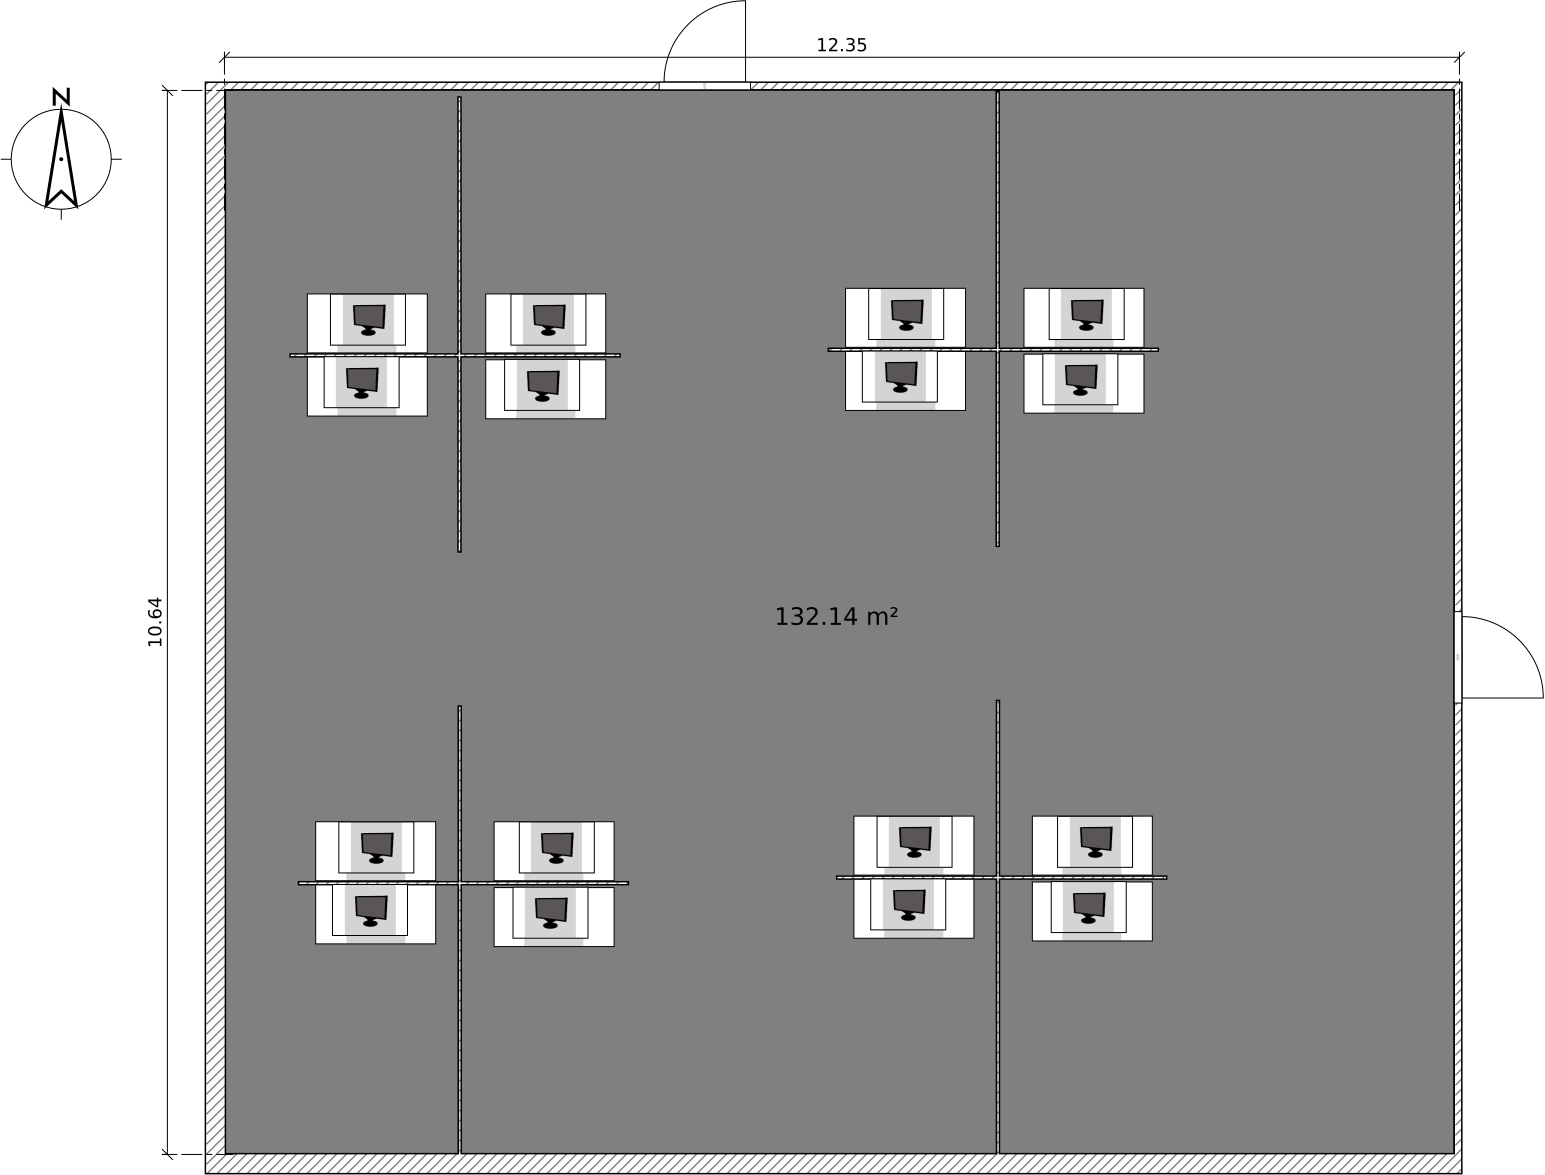
\includegraphics[scale=0.7]{labour/lab-plan}
            \end{center}
            \caption{Схема робочого приміщення}
            \label{fig:lab-plan}
    \end{figure}

    Геометричні параметри приміщення: ширина - 12.35 м, довжина - 10.6 м, висота - 3.5 м. Площа - 130.91 м кв., обєм - 458.2 м куб.
    Передбачається розміщення 16 робочих місць обладнаних системними блоками та рідкокристалічними моніторами.

    Згідно ДНАОП 0.00-1.31-99\cite{lab-dnaop} на одного працюючого повинно припадати не менше 6 м кв. площі та не менше 20 м. куб. oб'єму.
    У приведеному приміщенні 16 робочих місць і тоді відповідні параметри становлять 8.18 м. кв площі та при висоті стелі 3.5 м -  28.64 м куб. об'єму,
    що задовільняє норму.

    Для оздоблення слід використовувати матеріали з коефіцієнтом покриття для стелі 0.7 - 0.8, для стін 0.5 - 0.6.
    Покриття підлоги повинно бути матовим з коефіцієнтом відбиття 0.3 - 0.5. Поверхня підлоги повинна бути рівною і неслизькою.

\subsection{Небезпечні та шкідливі фактори}
    \subsubsection{Мікроклімат}
    Параметри мікроклімату визначаються з ДСН 3.3.6.042-99\cite{lab-dsn42}. Категорія робіт - легка Ia - роботи, що виконуються сидячи і не потребують
    важкого фізичного навантаження. Робоче місце постійне. Тому мікроклімат у робочому приміщенні повинен відповідати наступним вимогам.
    \begin{enumerate}
        \item оптимальна температура в холодний період року - 22..24С, у теплий - 23..25С;
        \item оптимальна відносна вологість 60-40\%;
        \item оптимальна швидкість руху повітря - 0.1 м/с.
    \end{enumerate}

    Для підтримки необхідної температури в холодний період року приміщення повинно бути облаштоване системою водяного центрального опалення з низьким тиском,
    а в теплий період року - системою кондиціонування -  спліт-система з внутрішнім блоком касетного типу.
    Так як вікна приміщення орієнтовані на схід, для уникнення перегрівання приміщення в літній період зранку, вікна повинні бути облаштовані жалюзями.

    \subsubsection{Освітлення}
    Освітлення у приміщенні здійснюється як за допомогою природних, так і за рахунок штучних джерел.
    Згідно ДБН В.2.5-28-2006\cite{lab-dbn28} сумарне освітлення робочої зони має бути таким, що сумарна освітленість на поверхні робочого столу становила 300-500 лк(для розряду зорових робіт Ia).

    Природнє освітлення здійснюється за рахунок вікон орієнтованих на схід, загальною площею 21 м кв.
    Штучне освітлення має здійснюватись переважно системою загального рівномірного освітлення -  люмінесцентними лампами типу ЛБ - 32 лампи
    ЛБ-18 G13 потужністю 18 Вт із застосуванням 8 світильників типу ЛВО(по 4 лампи) з зеркальними гратками.
    Система загального освітлення повинна становити лінії світильників, розташованих збоку від робочих місць, паралельно лінії зору працюючих.

    \subsubsection{Шум}
        Згідно ДСН 3.3.6.037-99\cite{lab-dsn37} рівень шуму та рівні звукового тиску для програмістів та вчених (творчі професії), мають бути не більше 50 дБA. 
        На робочому місці основними джерелами шуму є власний компютер та компьютери сусідів з еквівалентим рівнем шуму одного - 40 дБА, що в сумі дає 46 дБА
        і задовільняє норму.
        Еквівалентні рівні звукового тиску, що створює система кондиціонування повітря, повинні бути на 5 дБА менші.
    \subsubsection{Випромінювання}
    Рівні максимального електромагнітного випромінювання показані у таблиці\ref{tab:lab-waves}, причому максимальне значення
    електростатичного поля не повинно перевищувати 20 кВ/м.

    \begin{table}[h]
        \caption{Максимальні допустимі значення електромагнітного випромінювання на робочому місці}
        \begin{tabularx}{\textwidth}{| X | X | X |}
            \hline
            Напруженність & Електрична складова(В/м) & Магнітна складова(А/м) \\ \hline
            60 кГц до 3 мГц     & 50                       & 5                      \\ \hline
            3 кГц до 30 мГц     & 20                       & -                      \\ \hline
            30 кГц до 50 мГц    & 10                       & 0.3                    \\ \hline
            30 кГц до 300 мГц   & 5                        & -                      \\ \hline
        \end{tabularx}
        \label{tab:lab-waves}
    \end{table}

\subsection{Електробезпeка}
    Характер виконуваних у приміщенні робіт пов'язаний з постійним використанням електроустановок(системних блоків, моніторів), а тому необхідно забезпечити
    достатній рівень електробезпеки. Приміщення відноситься до класу без підвищеної небезпеки. Напруга у мережі становить 220В.

    Усі заземлені конструкції в приміщенні (батареї обігріву, водопровідні труби, кабелі з заземленим відкритим каналом),
    повинні бути захищені діелектричними щитками або сітками для недопущення потрапляння працівника під напругу. Для всієї проводки необхідно використовувати
    подвійну ізоляцію - основну та захисний короб.

    Необхідно забезпечити виконання наступних умов: усе обладнання в приміщенні повинно мати захист від короткого замикання та інших аварійних режимів,
    обладнання повинно підключатися виключно справними штепселями до стандартних електророзеток, лінія електромережі повинна бути окремою груповою трьохпроводною мережею, що складається
    з фазового, нульового робочого та нульового захисного провідників. Нульовий захисний провідник використовується для заземлення обладнання.


    \subsection{Пожежна безпека}
    Забезпечення пожежної безпеки у приміщенні повинно здійснюватися комплексом заходів: організаційних, системи виявлення пожеж та системи пожежогасіння.
    До пожежонебезпечних матеріалів у розглянутому приміщенні можна віднести - тверді горючі речовини(дерев'яні меблі - столи, шафи).
    Тоді згідно НАПБ Б.03.002-2007\cite{lab-napb} таке приміщення відноситься до категорії В(пожежонебезпечна).  Можливі пожежі - класу А(горіння твердих речовин), та класу Е - горіння електроустановок.

Приміщення повинно відповідати вимогам системи попередження пожеж (максимальне використання негорючих матеріалів, застосування аварійного відключення
на електроустановках, наявність систем виявлення пожежі, вогнегасників).
Так як основні причини пожежі у приміщенні пов'язані з електрикою(причому напруга не перевищує 380м), необхідно встановити автоматичну
дренчерну систему газового пожежогасіння з використанням хладона. Система повина бути обладнана димовими датчиками сповіщення про пожежу у кількості
не менше трьох.

\subsection{Техніка безпеки до виконання робіт}

    Роботи проводяться з використанням комп'ютера - пристрою, що працює під напругою. До виконання робіт допускаються виключно особи, що ознайомлені з усіма правилами безпеки.
    
    Перед початком робіт слід впевнитися, що робоче місце в порядку, а у приміщенні немає проблем з електрикою.
    Заборонено включати електроприбори, якщо на робочому місці присутня волога(наприклад, розлита вода).
    Якщо під час включення комп'ютера виникли іскри або дим, слід негайно виключити електричний рубильник,
    при необхідності скористатися вогнегасником, та сповістити про це спеціальні служби.
    Не слід самостійно переключати будь-які запчастини, переєднувати проводи - це повинен робити фахівець.
    При наявності відкритої проводки не слід розпочинати роботу.
    Не допускається наявність їжі та напоїв на робочому місці через загрози потрапляння води до електричних мереж.

% \section*{Висновки}
% \addcontentsline{toc}{section}{Висновки}
\newpage
\bigpart{Висновки}

\TBD
\bibliographystyle{gost71s}
\bibliography{myrefs}

\include{pz1/howto}
\end{document}
